\section{Van der Waerden's Theorem}

The rest of this chapter is motivated by the following question: if I $r$-colour the natural numbers $\N$, must I be able to find arbitrarily long monochromatic arithmetic progressions?

\begin{boxdefinition}[van der Waerden's Number]
    For $k, r \in \N$, the \textbf{van der Waerden number for $k$ and $r$}, denoted $\VW(k, r)$, is the least $N$ such that any $r$-colouring of $[N]$ admits a $k$-term monochromatic arithmetic progression.
\end{boxdefinition}

We will eventually show the following.

\begin{boxtheorem}[van der Waerden's Theorem] \label{Ch6:Thm:Van_Der_Waerden}
    For all $k, r \in \N$, $\VW(k, r)$ exists.
\end{boxtheorem}

$\VW(2, r) = r + 1$ is fairly straightforward. But what about $\VW(3, 2)$?

\subsection{Colour-Focusing}

% The seven provenance markers of the 30 September lecture below were carried over from the author's local copy of it (Local_Collective/lectures_28_30_sept.tex), which the Overleaf copy had dropped.
We can show that $\VW(3, 2) \geq 9$, because of the colouring
% [FILLED] the colours of $1, \ldots, 8$ are the standard extremal colouring, supplied here as the photo of the board does not show them
\begin{align*}
    \textcolor{red!75!black}{1} \quad \textcolor{red!75!black}{2} \quad \textcolor{blue!70!black}{3} \quad \textcolor{blue!70!black}{4} \quad \textcolor{red!75!black}{5} \quad \textcolor{red!75!black}{6} \quad \textcolor{blue!70!black}{7} \quad \textcolor{blue!70!black}{8} \quad 9
\end{align*}
where the minute you hit $9$ you get a monochromatic AP: $1, 5, 9$ if $9$ is red, and $7, 8, 9$ if $9$ is blue. (The choices previously were to try and minimise the chance of getting a $3$-term AP.)

We can also show that $\VW(3, 2) \leq 325$. How?

Write out blocks of five as follows:

\begin{figure}[h] % Note: This figure was generated by Claude
    \centering
    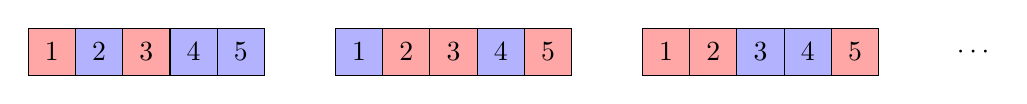
\begin{tikzpicture}[scale = 0.6]
        \foreach \b/\cols in {0/{red!35, blue!30, red!35, blue!30, blue!30}, 1/{blue!30, red!35, red!35, blue!30, red!35}, 2/{red!35, red!35, blue!30, blue!30, red!35}}{
            \foreach \c [count = \i] in \cols {
                \pgfmathsetmacro{\xpos}{6.5 * \b + \i - 1}
                \filldraw[fill = \c, draw = black] (\xpos, 0) rectangle ++(1, 1);
                \node at (\xpos + 0.5, 0.5) {$\i$};
            }
        }
        \node at (20, 0.5) {$\cdots$};
    \end{tikzpicture}
\end{figure}

(This is meant to represent a sequence of consecutive numbers, so the second box should really contain $6, 7, 8, 9, 10$, and so on. But this notation will prove convenient.)

We will essentially discover that when we have $65$ such boxes, any $2$-colouring of this sequence admits a monochromatic $3$-term AP.

Fix a $2$-colouring of this sequence. Notice that in any block of five, there is some $3$-term AP such that the first two terms are monochromatic. (Indeed, this is what motivates the choice of \textit{five} in the first place.)

We have a total of $2^5$ ways of colouring a block of five, so if we write down a total of $33 = 2^5 + 1$ blocks (which, in the worst case, consists of a block with each colour configuration, and then one more), we can always find two identically coloured blocks. Say these are the $i$th and the $j$th, with $i < j \leq 33$. Let $a, a + d, a + 2d \in \set{1, 2, 3, 4, 5}$ be the positions of their $3$-term AP, with $a$ and $a + d$ red, say.\footnote{Hence the notational convenience of using the same numbers, $1, 2, 3, 4, 5$, for each block.} If $a + 2d$ is also red, we're done, so suppose it is blue.

The intuition is to build an ``AP of blocks'' and use the next term after $i$ and $j$ to obtain the desired monochromatic $3$-term AP. Indeed, if we start at block $i$, this AP looks like $i + \ell (j - i)$. Going to the $\ell = 2$ term should give us the $(2j - i)$th block. Let's now show that this works.

Write $D = 5(j - i)$ for the distance between the two blocks, so that the $k$th element of block $j$ is exactly $D + (\text{the $k$th element of block $i$})$. In the $(2j - i)$th block, the $k$th element is exactly $D$ away from the $k$th element of block $j$. Now denote by $x$ the $(a + 2d)$th element of the $(2j - i)$th block.
\begin{description}
    \item[\underline{$x$ is red.}] Then position $a$ of block $i$, position $a + d$ of block $j$ and $x$ form a red AP with difference $D + d$.
    \item[\underline{$x$ is blue.}] Then position $a + 2d$ of blocks $i$, $j$ and $2j - i$ form a blue AP with difference $D$. (Remember, blocks $i$ and $j$ are coloured identically, and since the $(a + 2d)$th element of block $j$ is blue, so is that of $i$.)
\end{description}
Since $2j - i \leq 2 \cdot 33 - 1 = 65$, it suffices to have $65$ blocks of five, ie, $5 \cdot 65 = 325$ numbers.

We will now apply this technique to find a general upper-bound for van der Waerden numbers, and thereby, show they always exist (ie, prove van der Waerden's theorem).

We want to emphasise the concept of \textit{colour-focusing}: in our previous example, we saw that there were two APs that agreed at the last term, that were monochromatic until that one last ``focus'' term was coloured. That colouring would extend one of them but not the other. We thus make the following definition.

% [CORRECTED] was: each AP is monochromatic, except (possibly) at the $k$th term; all the APs have a common $k$th term (the focus point) --- the focus point is now the $(k + 1)$th term, so that the monochromatic AP in the definition of $\CF$ has one more term than the monochromatic part of each colour-focused AP
\begin{boxdefinition}[Colour-Focused APs]
    A collection of $k$-term APs is \textbf{colour-focused} if the following both hold:
    \begin{itemize}
        \item each AP is monochromatic
        \item all the APs have a common $(k + 1)$th term
    \end{itemize}
    The common $(k + 1)$th term of a family of colour-focused APs is called their \textbf{focus point}.
\end{boxdefinition}

The focus point could be the same colour as one of the APs, but it does not have to be. For our purposes, we will be interested in colour-focused APs that are different colours.

Let's now try and repeat the $\VW(3, 2)$ argument to find an upper-bound for $\VW(3, 3)$.

Divide the natural numbers into blocks of $7$. Again, our choice is motivated by the pigeonhole principle: for any $3$-colouring of all the numbers, any $7$-block admits a $3$-term AP such that the first $2$ terms are monochromatic.

\begin{figure}[H]
    \centering
    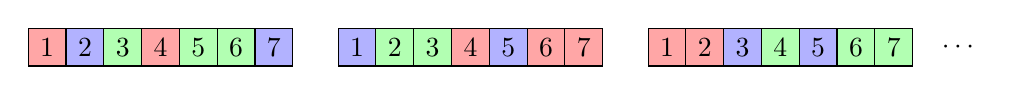
\begin{tikzpicture}[scale = 0.48]
        \foreach \b/\cols in {0/{red!35, blue!30, green!30, red!35, green!30, green!30, blue!30}, 1/{blue!30, green!30, green!30, red!35, blue!30, red!35, red!35}, 2/{red!35, red!35, blue!30, green!30, blue!30, green!30, green!30}}{
            \foreach \c [count = \i] in \cols {
                \pgfmathsetmacro{\xpos}{8.2 * \b + \i - 1}
                \filldraw[fill = \c, draw = black] (\xpos, 0) rectangle ++(1, 1);
                \node at (\xpos + 0.5, 0.5) {$\i$};
            }
        }
        \node at (24.6, 0.5) {$\cdots$};
    \end{tikzpicture}
\end{figure}

We have a total of $3^7$ ways of colouring a block, so if we write down $3^7 + 1 = 2188$ blocks, there are bound to be two that are identically coloured. As before, if we double this number and subtract one, ie, if we have $2\parenth{3^7 + 1} - 1 = 4375$ blocks, then we are guaranteed to have two colour-focused APs with a focus point.

The problem is that this focus point could take \textit{three} values, but as we only have two monochromatic APs, if it takes the colour not taken by the two APs, we do not have a monochromatic $3$-term AP.

What we have shown above is that if we have a total of $4375$ blocks, that is, $7 \cdot 4375$ numbers, we are guaranteed to have two APs with a shared focus point, which may or may not complete them.

To get three colour-focused APs, we need to ``go up one level'' and treat blocks of $7 \cdot 4375 = 30625$ numbers the way we treated blocks of $7$ to get two colour-focused APs. By the above, each such block contains either a monochromatic $3$-term AP, in which case we're done, or two colour-focused APs of different colours, say red and blue, whose focus point is green. There are $3^{30625}$ ways of colouring a $30625$-block, so among $3^{30625} + 1$ of them, two are identically coloured, say the $i$th and the $j$th. Write $\Delta = 30625(j - i)$, and let $y$ be the element of the $(2j - i)$th block in the same position as the focus point. We now have three APs heading for $y$:
\begin{itemize}
    \item the red AP, with its first term taken from block $i$ and its second from block $j$;
    \item the blue AP, likewise;
    \item the focus point of block $i$ followed by the focus point of block $j$, both green.
\end{itemize}

\begin{figure}[H] % Note: this diagram was generated by Claude
    \centering
    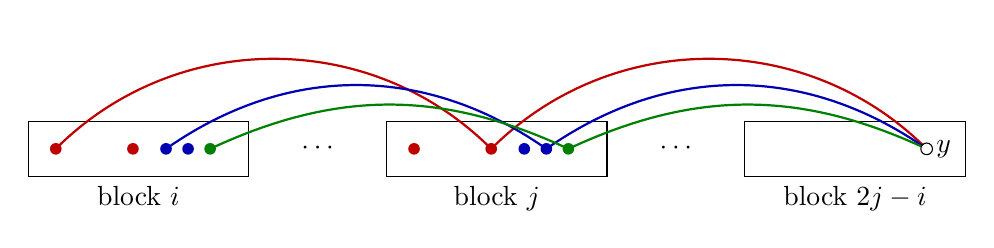
\begin{tikzpicture}[scale = 0.7]
        \foreach \x/\lab in {0/i, 6.5/j, 13/2j - i}{
            \draw (\x, 0) rectangle ++(4, 1);
            \node[below] at (\x + 2, 0) {block $\lab$};
        }
        \node at (5.25, 0.5) {$\cdots$};
        \node at (11.75, 0.5) {$\cdots$};
        \draw[red!75!black, thick] (0.5, 0.5) to[bend left = 45] (8.4, 0.5) to[bend left = 45] (16.3, 0.5);
        \draw[blue!70!black, thick] (2.5, 0.5) to[bend left = 35] (9.4, 0.5) to[bend left = 35] (16.3, 0.5);
        \draw[green!50!black, thick] (3.3, 0.5) to[bend left = 25] (9.8, 0.5) to[bend left = 25] (16.3, 0.5);
        \foreach \x in {0, 6.5}{
            \foreach \p/\c in {0.5/red!75!black, 1.9/red!75!black, 2.5/blue!70!black, 2.9/blue!70!black, 3.3/green!50!black}{
                \fill[\c] (\x + \p, 0.5) circle (3pt);
            }
        }
        \filldraw[fill = white, draw = black] (16.3, 0.5) circle (3pt) node[right] {$y$};
    \end{tikzpicture}
\end{figure}

Each of these is monochromatic, they have different colours, and each continues to $y$: if $p, q$ is an AP in block $i$ whose next term is the focus point $f$, then $p$ and $q + \Delta$ form an AP whose next term is $f + 2\Delta = y$. So these are three colour-focused APs of different colours, and whatever the colour of $y$, it completes one of them to a monochromatic $3$-term AP. As before, it suffices to have $2\parenth{3^{30625} + 1} - 1$ blocks of $30625$ numbers, so
\begin{align*}
    \VW(3, 3) \leq 30625 \cdot \parenth{2 \cdot 3^{30625} + 1}
\end{align*}

Not only have we found a bound on $\VW(3, 2)$ and $\VW(3, 3)$, we've also shown they \textit{exist}. We can actually use the strategy above to prove van der Waerden's Theorem (\Cref{Ch6:Thm:Van_Der_Waerden}).

\subsection{Colour-Focus Numbers}

First, a general definition.

% [CORRECTED] was: $s$ colour-focused $k$-term APs --- the focus can only be trapped if the APs have different colours (cf. the remark after the definition of colour-focused APs) and the focus point lies in $[N]$, so that it is coloured
\begin{boxdefinition}[Colour-Focus Number]
    For $k, r, s$ with $s \le r$, define the \textbf{colour-focus number} $\CF(k, r, s)$ to be the least $N$ such that any $r$-colouring of $[N]$ has either a monochromatic $(k + 1)$-term AP or $s$ colour-focused $k$-term APs of different colours, with focus point in $[N]$.
\end{boxdefinition}

We can bound van der Waerden numbers above by colour-focus numbers as follows.

\begin{boxlemma}\label{Ch6:Lemma:VW_le_CF}
    For all $k, r \in \N$,
    \begin{align*}
        \VW(k, r) \le \CF(k-1, r, r)
    \end{align*}
\end{boxlemma}
\begin{proof}
    Let $N = \CF(k-1, r, r)$. We need to show that any $r$-colouring of $[N]$ contains a $k$-term monochromatic arithmetic progression. But by definition of the colour-focus number, either $[N]$ admits a $k$-term monochromatic arithmetic progression (in which case we're done) or $r$ colour-focused $(k - 1)$-term arithmetic progressions. As we argued above, if there are $r$ such APs, then the focus must complete one of them, as we are $r$-colouring. So again we're done.
\end{proof}

We now prove a recursive bound on the colour-focus numbers.
% [CORRECTED] the proof below was re-indexed to match: a $(k - 1)$-term AP of blocks became a $k$-term one, $j \leq k - 1$ became $j \leq k$, and the focus block $B_{a + (k - 1)d}$ became $B_{a + kd}$; the sentence on the colour of the AP of focus points was added, as was ``of different colours'' in its first and last paragraphs, and ``for $k \geq 2$'' in the footnote

% [CORRECTED] was: For all $k, r, s \in \N$, with $\VW\of{k - 1, \cdot}$ --- $\CF(k, r, s - 1)$ needs $s \geq 2$, $\CF(k, r, s)$ needs $s \leq r$, and stretching APs with $k$ monochromatic terms needs $k$ identically coloured blocks, ie $\VW\of{k, \cdot}$
\begin{boxlemma}\label{Ch6:Lemma:CF_Recursion}
    For all $k, r, s \in \N$ with $2 \leq s \leq r$,
    \begin{align*}
        \CF(k, r, s)
        \leq \CF(k, r, s - 1) \cdot 2 \VW\of{k, r^{\CF\of{k, r, s - 1}}}
    \end{align*}
\end{boxlemma}
\begin{proof}
    Fix an $N \in \N$ and an $r$-colouring of $[N]$. Let $C = \CF\of{k, r, s - 1}$. Consider blocks in $[N]$ of length $C$. If any of them contains a $(k + 1)$-term monochromatic arithmetic progression, we're done, so assume that they all contain $(s - 1)$ $k$-term colour-focused arithmetic progressions of different colours. As they are all of length $C$, they must all have one property or the other.
    
    Each block can be coloured in one of $r^C$ ways. If we took $\VW\of{k, r^C}$ many blocks, say $B_1, \ldots, B_{\VW\of{k, r^C}}$, by definition of $\VW$, we would be able to find a $k$-term ``arithmetic progression of blocks''
    \begin{align*}
        B_{a}, B_{a + d}, B_{a + 2d}, \ldots, B_{a + (k - 1)d}
    \end{align*}
    that are all identically coloured.\footnote{We can ``code APs of blocks as APs'', and in this coding, a sequence of numbers being monochromatic translates to blocks being identically coloured.} If we take $2\VW\of{k, r^C}$ blocks\footnote{For $k \geq 2$, $2\VW\of{k, r^{\CF(k, r, s - 1)}} - 1$ would suffice, and we can even get tighter bounds, but the expression looks nicer without the ${} - 1$.}, we also have the focus block $B_{a + kd}$.

    What are some properties of this focus block? We know that it may not be coloured identically to the others in the AP of blocks. However, every block (APs and focus alike) has exactly $C$ elements, so each block contains $(s - 1)$ $k$-term colour-focused APs. Then, the families of APs that looks like ``the $j$th term of the $j$th block'', I get an AP with a focus point in $B_{a + kd}$. Ie, suppose my $(s - 1)$ $k$-term APs are denoted $\parenth{x^i_j}_{1 \leq j \leq k}$ for $1 \leq i \leq s - 1$, then I can build new APs $\parenth{y^i_j}_{1 \leq j \leq k}$ where for each $i$ in my family, I define $y^i_j$ to be the instance of $x^i_j$ living in the $j$th block $B_{a + (j - 1)d}$. This gives me $(s - 1)$ colour-focused APs in my set of numbers from the $2\VW\of{k, r^C}$ blocks (the focus point being the element of the focus block occupying the position of the focus points in the other blocks). Moreover, when I take the AP consisting of all the focus points, I get yet another AP with the same focus point as the $\parenth{y^i_j}$. Its colour is different from theirs: the $\parenth{y^i_j}$ have the colours of the $\parenth{x^i_j}$, and if the focus point of $B_a$ had the same colour as one of the $\parenth{x^i_j}$, the two together would form a monochromatic $(k + 1)$-term AP, which we have ruled out. Thus, I get a total of $s$ colour-focused APs.
    
    \begin{figure}[h] % Note: this diagram was generated by Claude
        \centering
        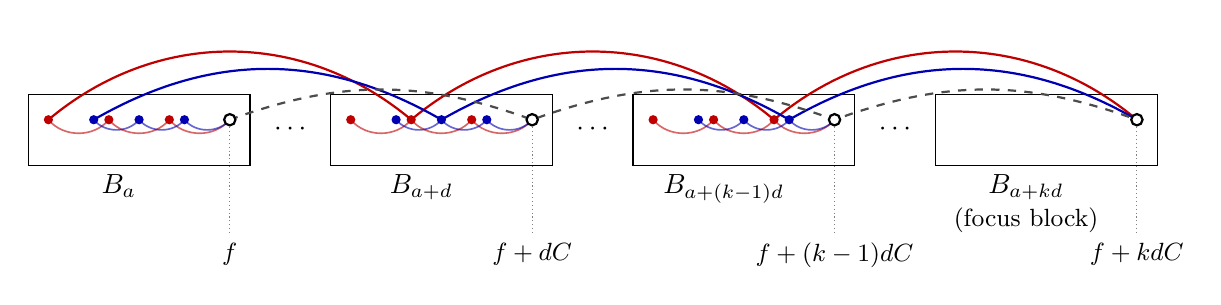
\begin{tikzpicture}[scale = 0.64]
            \foreach \x/\lab in {0/a, 6/a + d, 12/a + (k - 1)d, 18/a + kd}{
                \draw (\x, 0) rectangle ++(4.4, 1.4);
                \node[below] at (\x + 1.8, 0) {$B_{\lab}$};
            }
            \node at (5.2, 0.7) {$\cdots$};
            \node at (11.2, 0.7) {$\cdots$};
            \node at (17.2, 0.7) {$\cdots$};
            \node[below] at (19.8, -0.65) {\small (focus block)};
            % inside each identically coloured block: the s - 1 colour-focused APs, running into that block's focus point
            \foreach \x in {0, 6, 12}{
                \draw[red!75!black, semithick, opacity = 0.6] (\x + 0.4, 0.9) to[bend right = 50] (\x + 1.6, 0.9) to[bend right = 50] (\x + 2.8, 0.9) to[bend right = 50] (\x + 4, 0.9);
                \draw[blue!70!black, semithick, opacity = 0.6] (\x + 1.3, 0.9) to[bend right = 50] (\x + 2.2, 0.9) to[bend right = 50] (\x + 3.1, 0.9) to[bend right = 50] (\x + 4, 0.9);
            }
            % across blocks: the stretched APs, and the AP of focus points
            \draw[red!75!black, thick] (0.4, 0.9) to[bend left = 40] (7.6, 0.9) to[bend left = 40] (14.8, 0.9) to[bend left = 40] (22, 0.9);
            \draw[blue!70!black, thick] (1.3, 0.9) to[bend left = 30] (8.2, 0.9) to[bend left = 30] (15.1, 0.9) to[bend left = 30] (22, 0.9);
            \draw[black!70, thick, dashed] (4, 0.9) to[bend left = 20] (10, 0.9) to[bend left = 20] (16, 0.9) to[bend left = 20] (22, 0.9);
            \foreach \x in {0, 6, 12}{
                \foreach \p/\c in {0.4/red!75!black, 1.6/red!75!black, 2.8/red!75!black, 1.3/blue!70!black, 2.2/blue!70!black, 3.1/blue!70!black}{
                    \fill[\c] (\x + \p, 0.9) circle (2.6pt);
                }
            }
            % the focus points, hollow, labelled underneath the diagram
            \foreach \x/\lab in {0/f, 6/f + dC, 12/f + (k - 1)dC, 18/f + kdC}{
                \filldraw[fill = white, draw = black, thick] (\x + 4, 0.9) circle (3.2pt);
                \draw[black!50, densely dotted] (\x + 4, 0.75) -- (\x + 4, -1.35);
                \node[below] at (\x + 4, -1.35) {\small $\lab$};
            }
        \end{tikzpicture}
    \end{figure}

    The total number of elements living in my $2\VW\of{k, r^C}$ blocks is $C \cdot 2\VW\of{k, r^C}$. So effectively, when $N = C \cdot 2\VW\of{k, r^C}$, any $r$-colouring of $[N]$ admits either a $(k + 1)$-term monochromatic AP or $s$ colour-focused $k$-term APs of different colours. Thus, this value of $N$ is an upper-bound on $\CF\of{k, r, s}$.
\end{proof}

We can use our recursive bound on colour-focus numbers to prove that colour-focus numbers always exist\footnote{Maybe you need to choose $k, r, s$ so that $\CF(k, r, s)$ actually makes sense, but we won't split hairs about this.}. This ultimately tells us that van der Waerden numbers also always exist.

\begin{boxtheorem}
    $\CF(k, r, s)$ always exists.
\end{boxtheorem}
\begin{proof}
    % [CORRECTED] the base case below gained the pigeonhole step, needed now that colour-focused APs must have different colours
    Proceed by induction on $k$, keeping $r$ and $s$ generic\footnote{In Lean this would be \lstinline|induction k generalizing r s|.}. When $k = 1$, the result is trivial, because no matter the value of $r$ or $s$, if we consider the set $[s + 1]$, we can always find either a $2$-term monochromatic AP (ie, two numbers with the same colour) or $s$ $1$-term monochromatic colour-focused APs (ie, $s + 1$ numbers with distinct colours).

    Now fix $k$ and assume $\CF(k, r, s)$ exists for all $r, s$. We want to show that $\CF(k + 1, r, s)$ also exists for all $r, s$. We proceed by induction on $s$.

    $\CF(k + 1, r, 1)$ certainly always exists. In general, $\CF(a, b, 1)$ exists iff there is some $N \in \N$ such that any $b$-colouring of $[N]$ admits a monochromatic $a$-term AP. Take $N \geq \CF(k, r, r)$ (which exists by the induction hypothesis on $k$). Then either $[N]$ admits a $(k + 1)$-term monochromatic AP (in which case we're done) or $[N]$ admits $r$ colour-focused $k$-term APs (in which case the focus point extends one of them to a monochromatic $(k + 1)$-term AP, as there are precisely $r$ of them).

    % [CORRECTED] was: $\VW\of{k, \cdot}$ and $\CF\of{k - 1, \cdot, \cdot}$ below --- these follow the recursive bound's $\VW\of{k + 1, \cdot}$, and $\CF\of{k, \cdot, \cdot}$ is exactly the induction hypothesis on $k$
    Now fix $s$ and suppose $\CF(k + 1, r, s)$ exists for all $r$. Then by \Cref{Ch6:Lemma:CF_Recursion,Ch6:Lemma:VW_le_CF}, we know
    \begin{align*}
        \CF\of{k + 1, r, s + 1}
        &\leq \CF\of{k + 1, r, s} \cdot 2 \VW\of{k + 1, r^{\CF\of{k + 1, r, s}}} \\
        &\leq \CF\of{k + 1, r, s} \cdot 2 \CF\of{k, r^{\CF\of{k + 1, r, s}}, r^{\CF\of{k + 1, r, s}}}
    \end{align*}
    The above colour-focus numbers both exist by the induction hypotheses on $k$ and $s$, finishing the induction.
\end{proof}

\Cref{Ch6:Thm:Van_Der_Waerden} (van der Waerden's theorem) is an immediate corollary.

\subsection{A Lower Bound from the Local Lemma}

The bounds above are enormous. For comparison, here is what the \Lovasz{} local lemma (\Cref{Ch5:Cor:Symmetric_LLL}) gives from below.

% Not from the lecture: the lecture of 7 October quoted this bound as already shown, ``using the Lovasz Local Lemma'', and no earlier lecture in these notes shows it (chapter 5 states the lemma and proves nothing with it but the symmetric form). The statement and proof were supplied in answer to the author's ``when? where? how?''; the proof originally derived the symmetric form of the local lemma inline, and cites \Cref{Ch5:Cor:Symmetric_LLL} since 2026-10-08.
\begin{boxproposition} \label{Ch6:Prop:VW_Lower_Bound}
    For all $k \geq 2$,
    \begin{align*}
        \VW\of{k, 2} > \frac{(k - 1) \, 2^{k - 1}}{e k^2}
    \end{align*}
    In particular, $\VW\of{k, 2} = \Omega\of{\frac{2^k}{k}}$.
\end{boxproposition}
\begin{proof}
    Let $N = \floor{\frac{(k - 1) 2^{k - 1}}{e k^2}} + 1$. It suffices to find a $2$-colouring of $[N]$ with no monochromatic $k$-term arithmetic progression, as then $\VW(k, 2) > N$. If $N < k$ there is nothing to find, since $[N]$ has no $k$-term progressions at all, so assume $N \geq k$.

    Colour $[N]$ red or blue uniformly and independently at random. For each $k$-term arithmetic progression $P \ssq [N]$, let $A_P$ be the event that $P$ is monochromatic, so that $\Pr\of{A_P} = 2^{1 - k}$. $A_P$ is determined by the colours of the points of $P$ alone, so joining $A_P$ to $A_Q$ exactly when $P$ and $Q$ share a point gives a dependency graph. A progression through a given point is determined by its common difference, which is at most $\frac{N - 1}{k - 1}$, and by the position of the point in it, so a point lies in at most $\frac{k (N - 1)}{k - 1}$ progressions, and $A_P$ has at most
    \begin{align*}
        D = \frac{k^2 (N - 1)}{k - 1} - 1
    \end{align*}
    neighbours. Now
    \begin{align*}
        e \cdot 2^{1 - k} \parenth{D + 1} = \frac{e k^2 (N - 1)}{(k - 1) 2^{k - 1}} \leq 1
    \end{align*}
    by the choice of $N$, so \Cref{Ch5:Cor:Symmetric_LLL} applies, and with positive probability no $A_P$ occurs: some $2$-colouring of $[N]$ has no monochromatic $k$-term arithmetic progression.
\end{proof}
